%%% -*-LaTeX-*-

\chapter{SAT Encodings}

In this chapter we'll examine how the language forms we saw in the previous chapter are efficiently encoded as boolean formulas. A program in SweetPea is translated to a boolean formula in Conjunctive Normal Form (CNF), which is a canonicalization that is frequently used by SAT solvers and samplers. We use two techniques for efficient SAT encodings: we encode large "counting" constraints using a Tsietin transform, and user's derivation constraints more directly. After examining how a program is encoded, we'll also discuss the runtime communication with the sampler, and why the correctness guarantees are preserved.

\section{Conjunctive Normal Form (CNF)}

A boolean formula consists of boolean variables combined using boolean operators, such as \texttt{and}, \texttt{or} and \texttt{not}. There are many canonical forms for boolean formulas; the one that SAT solvers commonly use is Conjunctive Normal Form (CNF). CNF is an "and of ors". This means that CNF is built out of OR clauses, which are clauses in which the boolean OR operator is applied to a list of variables. \texttt{A or B or (not C) or D} is an example of an OR clause. CNF is then the AND operator applied to a list of OR clauses. \texttt{(A or B) and (C or not D)} is an example of a boolean formula in CNF.

SAT solvers typically process boolean formulas in CNF. This is partially because they are amenable to the search strategies that solvers commonly employ while searching for satisfying assignments, and partially because there is an efficient translation from a boolean formula in any form to the CNF canonical form.

More specifically, solvers typically process boolean formulas in the DIMACS CNF form. In the DIMACS convention, boolean variables are denoted by their index, and negation is denoted by a minus sign. This means that a formula like \texttt{(A or B) and (C or not D)} is represented as \texttt{(1 or 2) and (3 or -4)}. This index based renaming is very convinient as a convention for generating fresh variable names-- we just need to increment the variable counter to get a fresh variable. Each or-clause is written on an individual line, and every term within the or-clause is written as an element of a list; each list is terminated with the number 0. Finally, each formula also has a header which clues the consumer to the number of variables and clauses in formula. The full DIMACS CNF specification of the example in this paragraph is:
\begin{verbatim}
p cnf 4 2
1, 2, 0
3, -4, 0
\end{verbatim}

This specification is the langauge required to leverage the awesome power of SAT samplers and solvers, but it is clearly not amemable to being manually specified by human hands for anything but the most toy examples. That is why SweetPea provides a high-level domain-specific interface which compiles to these low-level specifications. An interesting aspect of the translation is ensuring that the encoding is efficeint: that is, polynomial in the number of number of variables and clauses with respect to the constraint size.

\section{Representing SweetPea Primitives in CNF}

Recall that experimental designs describe trials in terms of factors and levels, and the relationships between those trials in terms of windows, derivation functions and counting constraints. Here, let's see how all of those components are encoded into a boolean formula; in the next chapter we'll discuss trade-offs of some encoding decisions and more details.

\subsection{Representing Levels and Necessary Constraints}

\begin{figure}[t]
    \centerline{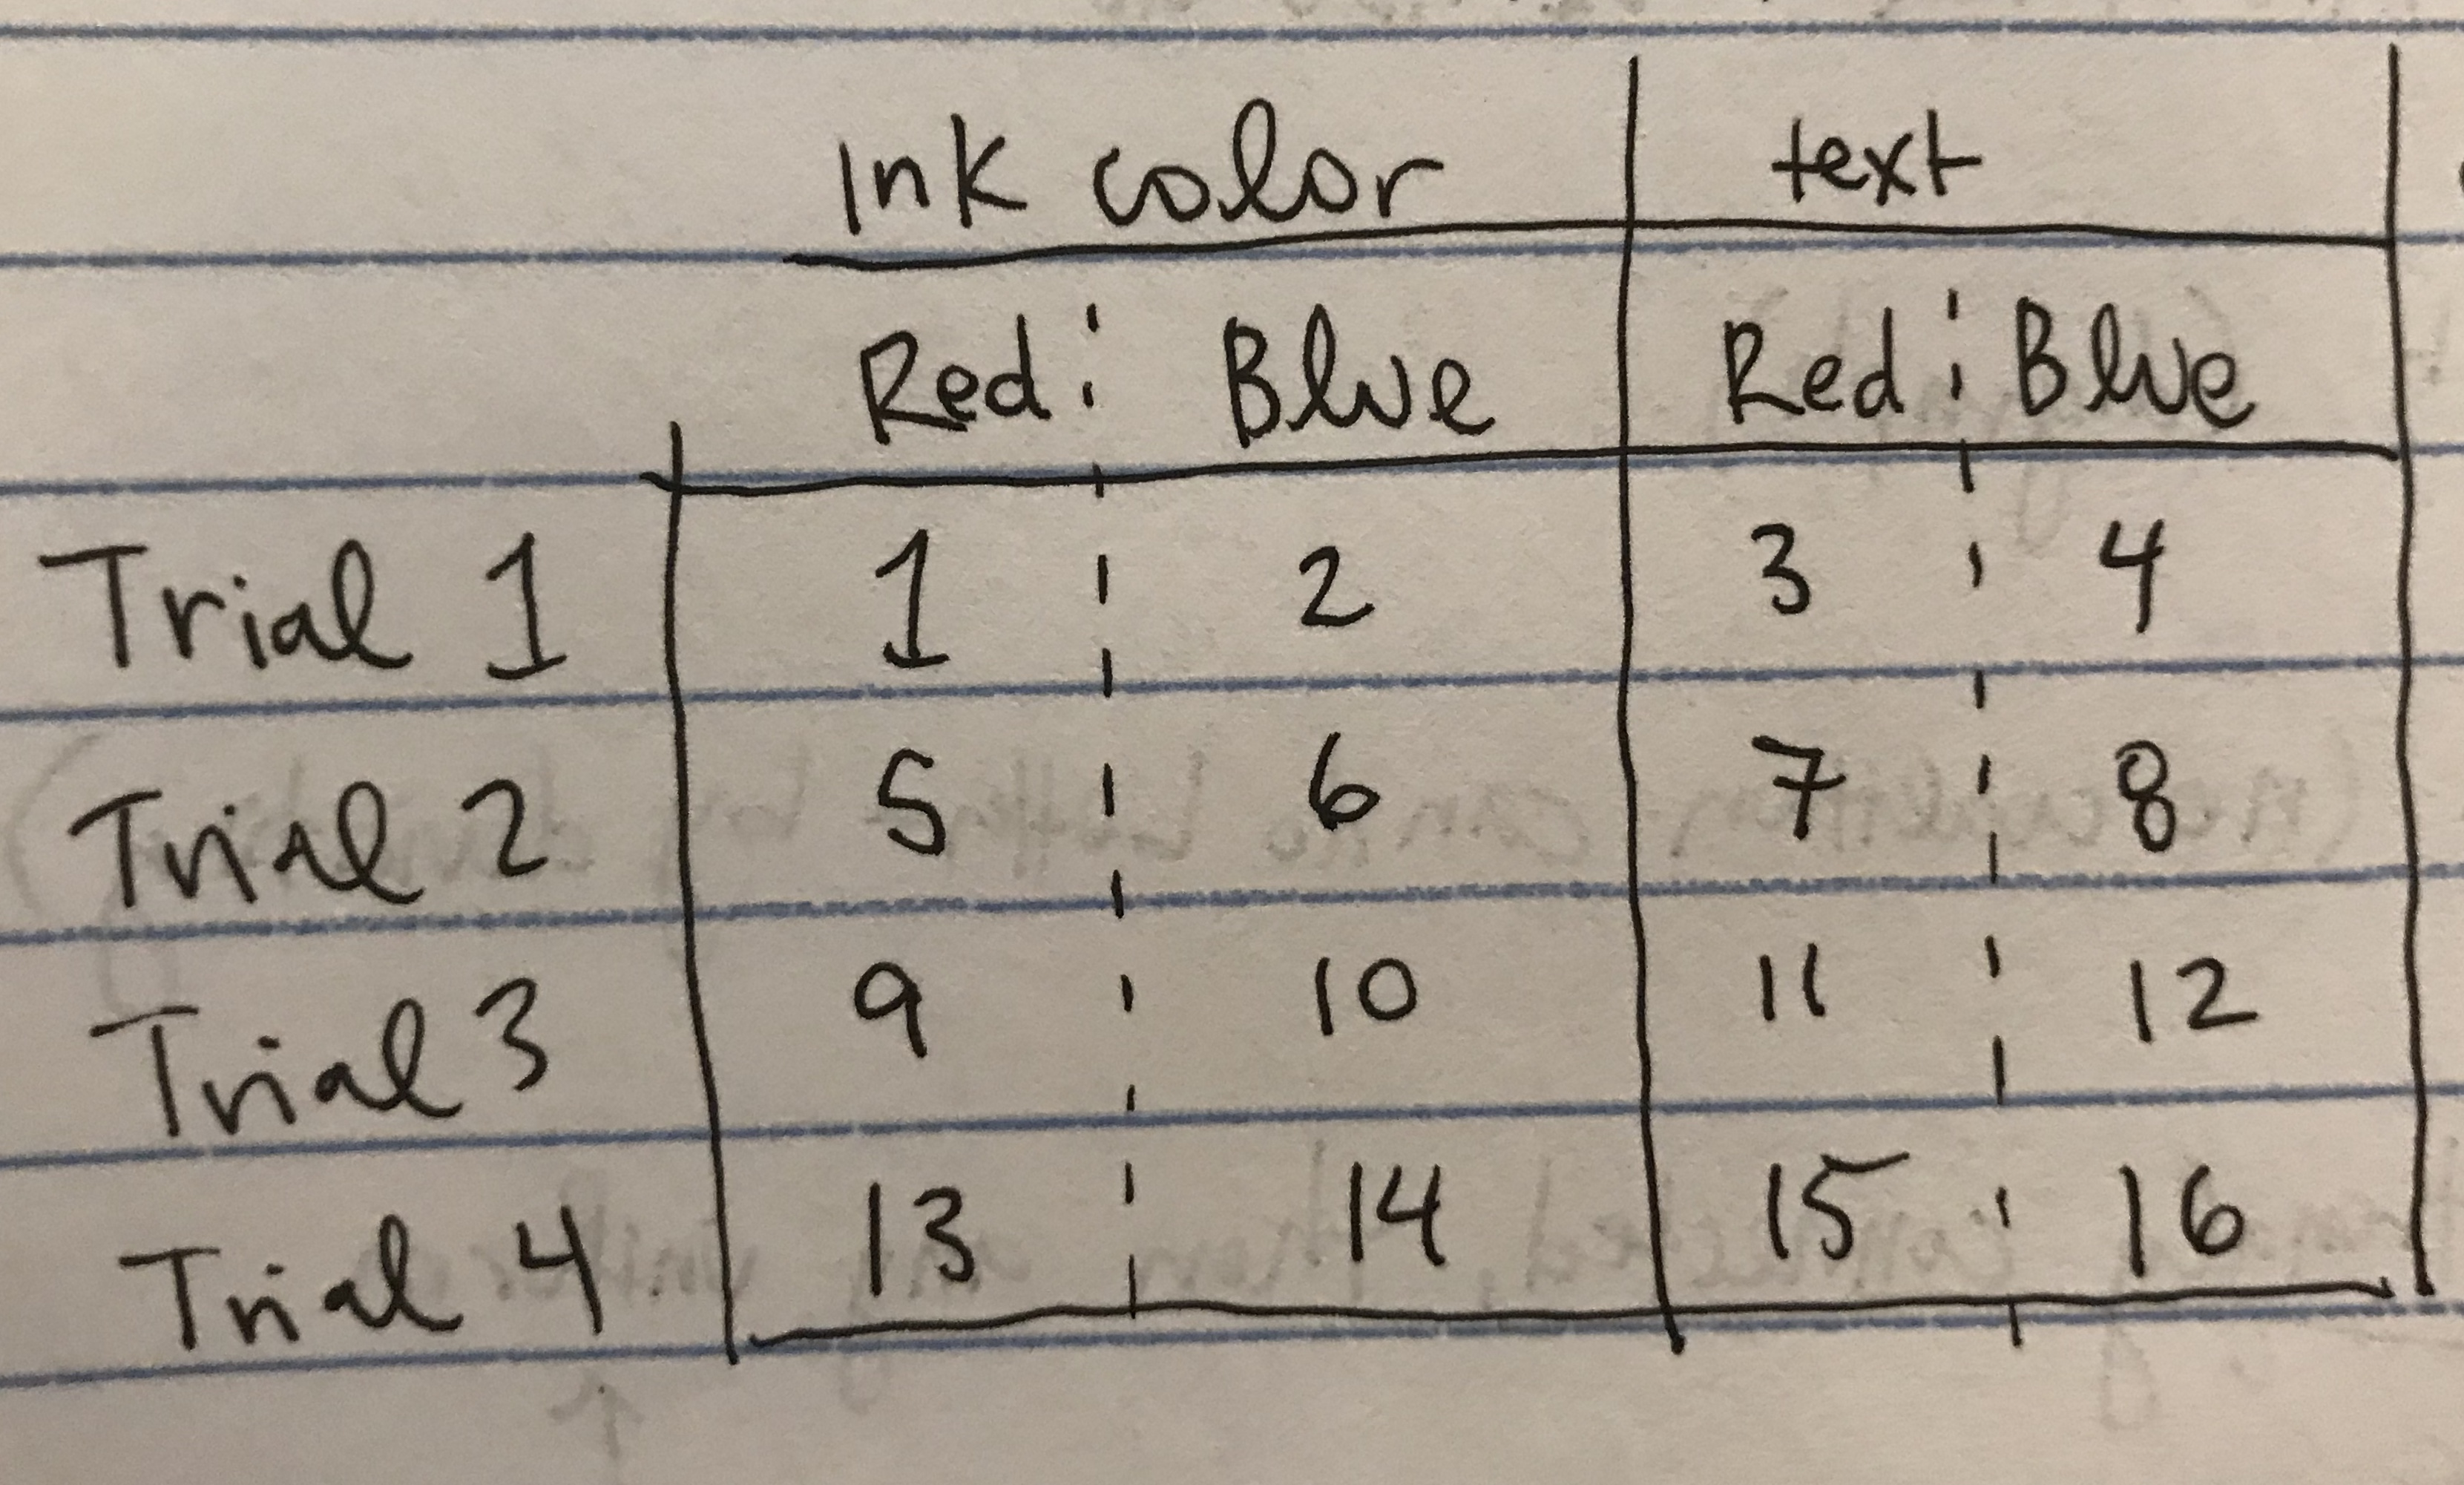
\includegraphics[origin=c,width=10cm]{encoding_strupe_vars}}
    \caption{Variable allocation for the running Stroop example.}%
    \label{fig:encoding_strupe_vars}%
\end{figure}

An experimental sequence consists of a specification for every trial in the experiment. Each trial is parameterized by factors, and the specification indicates which level of each factor is selected. Levels correspond naturally to boolean variables; a factor has one level at a time selected and each level can exist in either a selected state or a non-selected state.

The encoding we use allocates one boolean variable for each level of each factor of each trial. See figure \figref{encoding_strupe_vars} for a visualization of the variable allocation for the running Stroop example. In the running example, there are 4 trials, each of which is described by two factors with two levels. The encoding we use allocates one variable for every factor for every trial. As mentioned in the previous subsection, variables in the DIMACS CNF format are index-based, which means that the number 1 refers to the first boolean variable and so on. This means that the assignments to variables 1 through 4 represents the specification of the first trial. For instance, the assignment \texttt{1 -2 -3 4} means the ink color is red (and not blue), and the text is blue (and not red). For any experiment we allocate (total number of levels) * (number of trials) boolean variables which directly encode a specification of an experimental sequence.

\begin{figure}[t]
    \centerline{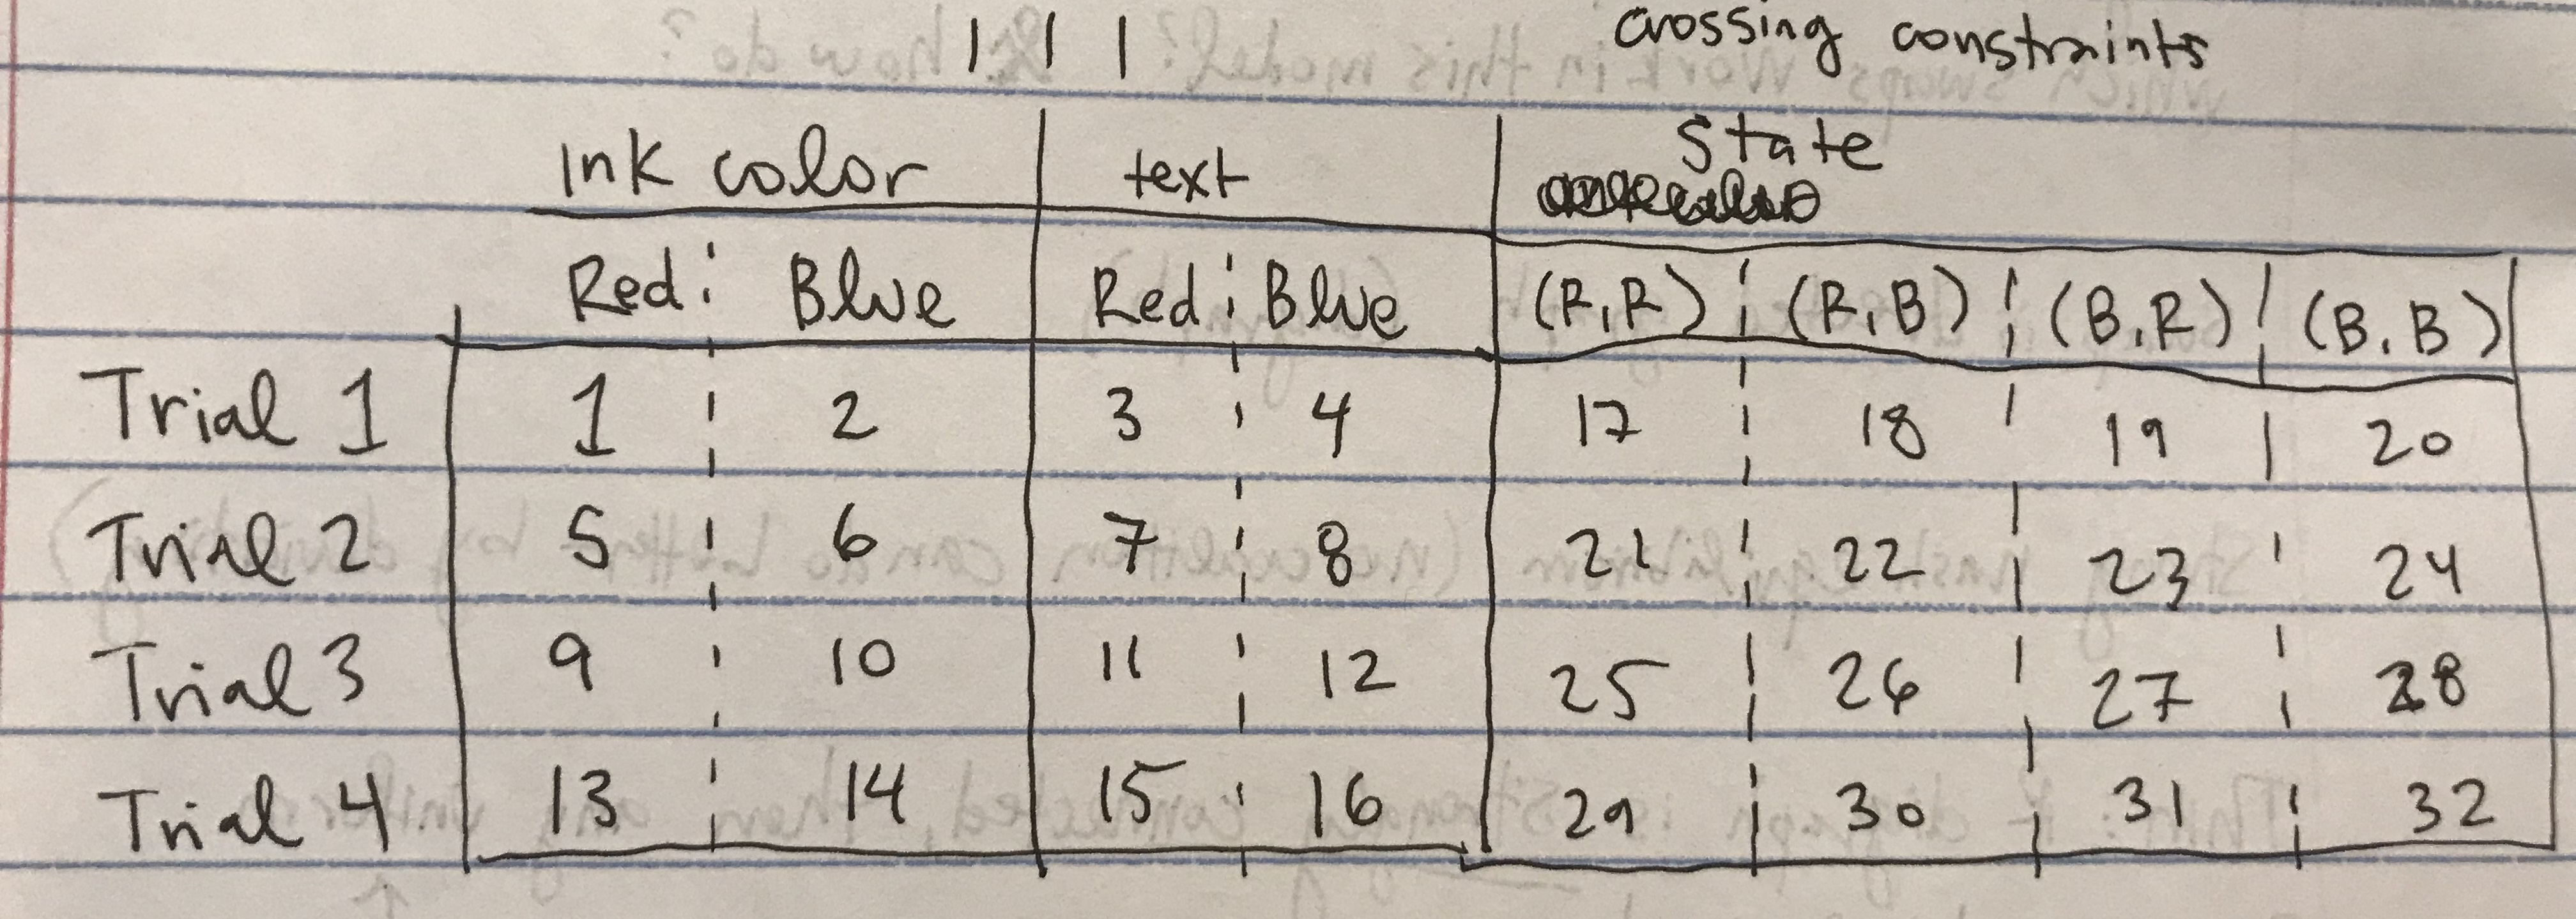
\includegraphics[origin=c,width=10cm]{stroop_crossing_vars}}
    \caption{Additional variable allocation necessary for encoding the states possible in the full crossing.}%
    \label{fig:stroop_crossing_vars}%
\end{figure}

There are two kinds of constraints which need to be encoded; user-defined constraints and two other constraints which are always necessary to correctly model the experiment. The first are \emph{consistency constraints} which state that only one level of each factor is selected at once. In the running example constraints of the form \texttt{(1 and not 2) or (not 1 and 2)} for each pair of levels would ensure that only one level is true at a time. The second kind of constraint is a \emph{crossing constraint} which ensures that the correct number of each kind of possible trial occurs in the experimental sequences.

Representing crossing constraints is more complicated. In the running example, the logic for the crossing constraints should ensure that there is one (red ink, red text), one (red ink, blue text), one (blue ink, red text) and one (blue ink, blue text). To do encode this, we allocate 4 more variables for each trial, each of which literally encodes which of those 4 states that trial represents. See figure \figref{stroop_crossing_vars} for a visualization of the additional variables. Let's look at the constraints we need to add for the first trial-- first we'll add a constraint that specifies that trial is in the (red ink, red text) state if-and-only-if the red ink level is selected, and the red text level is selected \texttt{(17 iff (1 and 3))}. We add constraints of this form for the other 3 states as well, ie \texttt{(18 iff (1 and 4))}, \texttt{(19 iff (2 and 3))}, \texttt{(20 iff (2 and 4))}. Next, we create constraints to ensure that exactly one of each of the state variables across all the trials is true, ie, (exactly one of 17, 21, 25, 29 is true), (exactly one of 18, 22, 26, 30 is true), and so on.

A realistic experiment may have on the order of 100 trials. This means that we need to be careful with this last constraint, that exactly one of \texttt{<}list of length 100\texttt{>}, is true. In other types of crossings (see chapter 4, section 4.2.3) that constraint may more generally be exactly k of \texttt{<}list of length 100\texttt{>} is true. The naive encoding (these k, or those k, or those k, and so on) is exponential, therefore not efficient, and in practice too large for our problem size. Instead, we efficiently encode these \emph{counting constraints} following a technique similar to the one described in \cite{sinz2005towards}. For a detailed description of this algorithm, see the next chapter.

In summary, an experimental sequence is represented as a list of boolean variables for each level of each trial. Assignments to these variables uniquely specify the experimental sequence. Irregardless of other user constraints, these variables are bound by constraints to ensure exactly one level is selected at a time for each factor, and that each state in the crossing is represented the correct number of times. The next chapter will examine the trade-offs from our encoding decisions. Next we'll see how these variables which represent levels can be used to encode derived levels and used with window constraints.

\subsection{Representing Derived Levels and Derivation Functions}

The current SweetPea implementation special-cases the constraint encoding for congruency and transitions because these are common constraints in the experiments we wish to model.

Let's consider a congruency derivation over the simple Stroop example. In addition to the variables which represent the levels of each trial, we'll allocate 2 new variables for each trial each of which indicates whether or not the trial is congruent. This means the variable allocation looks like:

\begin{verbatim}
----------------------------------------------
|   Trial |  color   |   text   | congruent? |
|       # | red blue | red blue |  con  inc  |
----------------------------------------------
|       1 |  1   2   |  3   4   |   5    6   |
|       2 |  7   8   |  9   10  |  11    12  |
|       3 | 13   14  | 15   16  |  17    18  |
|       4 | 19   20  | 21   22  |  23    24  |
----------------------------------------------
\end{verbatim}

Then, we encode constraints on when these new variables are true. When is the first trial congruent? The first trial (\texttt{5}) is congruent if-and-only-if either the trial's color is red (\texttt{1}) and the text is red (\texttt{3}), or the color is blue (\texttt{2}) and the text is blue (\texttt{2}). In boolean logic this is: \texttt{5 iff (1 and 3) or (2 and 4)}. We create constraints of this form for all the remaining variables, and translate this constraint to CNF through a general CNF conversion technique.

What if instead we considered transitions? Let's reinterpret the variable named \texttt{5} to indicate whether that trial has the same text as the following trial:

\begin{verbatim}
----------------------------------------------
|   Trial |  color   |   text   | transition |
|       # | red blue | red blue |  swi  rep  |
----------------------------------------------
|       1 |  1   2   |  3   4   |   5    6   |
|       2 |  7   8   |  9   10  |  11    12  |
|       3 | 13   14  | 15   16  |  17    18  |
|       4 | 19   20  | 21   22  |  23    24  |
----------------------------------------------
\end{verbatim}

We can then state that the trial switches (\texttt{5}) if-and-only-if this trial's text is red (\texttt{3}) and the next trial's text is also red (\texttt{9}), or they are both blue (\texttt{4} and \texttt{10}). In boolean logic this is: \texttt{5 iff (3 and 9) or (4 and 10)}. This identical clause structure allows us to model both of these common derivations. Encoding arbitrary derivations is left as future work.

\section{Correctness Guarantees}

The goal of SweetPea is to produce experimental sequences which satisfy the experimental design with uniform probability: not favoring any valid sequence over any other. SweetPea achieves this goal by relying on the uniform samping guarantee that Unigen provides in \cite{chakraborty2013scalable}.

Unigen is a near-uniform SAT sampler. Near-uniform is defined in \cite{meel2016constrained} as

\begin{align*}
  \frac{1}{\text{number of solutions}\times(1+ \epsilon)} & \leq \text{Probability[Finding a given solution]} \\
  &\leq (1+\epsilon) / \text{number of solutions}
\end{align*}

This guarantees that the number of \emph{SAT witnesses}, or satisfying solutions, to the CNF is approximately uniformly probable. How does the number of satisfying SAT solutions relate to the number of experimental sequences which satisfy the experimental design?

When we translate from the high level specification to the boolean formula, we introduce new internal boolean variables (ie the sum and carry bits of the adders in the popcount encoding). We hypothesize that the number of satisfying SAT solutions is exactly the same as the number of experiment sequences when none of the internal boolean variables are redundant. Then, all the variables which directly encode the experiment are in lockstep with all the extra internal variables. If there are redudant variables, they could skew the number of satisfying assignments such that finding an assignment would be uniform with those variables, but not in the variables we care about. To the best of our knowledge, our encoding does not introduce redundant variables, and therefore preserves this guarantee.
